%
%   Data description
%       - Importing data
%       - Data preprocessing
%       - Data cleaning
%   
\clearpage
\section{Data description}









\subsection{Overview of the dataset}

Write something about the dataset, because no one will understand what a chip is 
if we don't elaborate them.

Some parts from Importing data section could be brought to here.










\subsection{Importing data}
For the first part of our project, we need to select a suitable dataset for us to analyze, as we are computer science students, we have decided to select a CPU data set, the data of which can be found \href{https://www.kaggle.com/datasets/iliassekkaf/computerparts?select=Intel_CPUs.csv}{here}:
\\
The data give us information about 2283 CPU and 45 of their attribute which include:
\\
\begin{itemize}
    \item Product\_Collection: tell us which type of series the core belongs to.
    \item Vertical\_Segment: show what kind of system the CPU was designed for (embedded, mobile, desktop, or sever).
    \item Processor\_Number	: process ID.
    \item Status: show the status of the CPU (announce, launched, end of life, end of support).
    \item Launch\_Date: The date the product was first introduced. 
    \item Lithography: refers to the semiconductor technology used to manufacture an integrated circuit, and is reported in nanometers (nm), indicative of the size of attributes built on the semiconductor. 
    \item Recommended\_Customer\_Price: recommended customer price. 
    \item nb\_of\_Cores: total number of cores in a proccessor. 
    \item nb\_of\_Threads: total number of thread in a processor. 
    \item Processor\_Base\_Frequency: Describes the rate at which the processor's transistors open and close.
    \item Max\_Turbo\_Frequency: The maximum single core frequency at which the processor is capable of operating using Intel® Turbo Boost Technology. 
    \item Cache: CPU Cache is an area of fast memory located on the processor. 
    \item Bus\_Speed: refers to how much data can move across the bus simultaneously.
    \item TDP(thermal design power): Represents the average power, in watts, the processor dissipates when operating at Base Frequency with all cores. 
    \item Embedded\_Options\_Available: is it allow to be embedded system
    \item Conflict\_Free: Defined by the U.S. Securities and Exchange Commission rules to mean products that do not contain conflict minerals (tin, tantalum, tungsten).
    \item Max\_Memory\_Size: The maximum memory capacity supported by the processor. 
    \item Memory\_Types: Single Channel, Dual Channel, Triple Channel, and Flex Mode.The maximum memory capacity supported by the processor.
    \item Max\_nb\_of\_Memory\_Channels: The number of memory channels refers to the bandwidth operation for real world application.
    \item Max\_Memory\_Bandwidth: The maximum rate at which data can be read from or stored into a semiconductor memory by the processor (in GB/s). 
    \item ECC\_Memory\_Supported: ECC memory is a type of system memory that can detect and correct common kinds of internal data corruption.
    \item Processor\_Graphics: integrated graphics processing unit (GPU) that is built into some of Intel's processors.
    \item Graphics\_Base\_Frequency: The rated/guaranteed graphics render clock frequency in MHz.
    \item Graphics\_Max\_Dynamic\_Frequency: The maximum opportunistic graphics render clock frequency (in MHz) that can be supported using Intel HD Graphics with Frequency attribute.
    \item Graphics\_Video\_Max\_Memory: The maximum amount of memory accessible to processor graphics. Processor graphics operates on the same physical memory as the CPU (subject to OS, driver, and other system limitations).
    \item Graphics\_Output: Graphics Output defines the interfaces available to communicate with display devices.
    \item Support\_4k: indicates the product's support of 4K
    \item Max\_Resolution\_HDMI: the maximum resolution supported by the processor via the HDMI interface (24bits per pixel \&amp; 60Hz). System or device display resolution is dependent on multiple system design factors; actual resolution may be lower on your system.
    \item Max\_Resolution\_DP: The maximum resolution supported by the processor via the DP interface (24bits per pixel \&amp; 60Hz). System or device display resolution is dependent on multiple system design factors.
    \item Max\_Resolution\_eDP\_Integrated\_Flat\_Panel	
    \item DirectX\_Support: Indicates support for a specific version of DirectX, a Microsoft collection of APIs for handling multimedia compute tasks.
    \item OpenGL\_Support: Indicates support for OpenGL, a cross-language, multi-platform API for rendering 2D and 3D vector graphics. 
    \item PCI\_Express\_Revision: The PCIe version supported by the processor. 
    \item PCI\_Express\_Configurations\_: The available PCIe lane configurations that can be used to link the PCH PCIe lanes to PCIe devices.
    \item T : The maximum temperature allowed on the chip.
    \item Max\_nb\_of\_PCI\_Express\_Lanes: maximum number of PCI Express Lanes that are supported.
    \item Intel\_Hyper\_Threading\_Technology\_: Delivers two processing threads per physical core. Highly threaded applications can get more work done in parallel, completing tasks sooner.
    \item Intel\_Virtualization\_Technology\_VTx\_: Allows one hardware platform to function as multiple “virtual” platforms. It offers improved manageability by limiting downtime and maintaining productivity by isolating computing activities into separate partitions.
    \item Intel\_64\_: Delivers 64-bit computing on server, workstation, desktop and mobile platforms when combined with supporting software. Intel 64 architecture improves performance by allowing systems to address more than 4 GB of both virtual and physical memory.
    \item Instruction\_Set: Which instrution set the CPU use.
    \item Instruction\_Set\_Extensions :  Instruction set extension
    \item Idle\_States: Used to save power when the processor is idle.
    \item Thermal\_Monitoring\_Technologies: Protects the processor package and the system from thermal failure through several thermal management attributes.	
    \item Secure\_Key: The CPU is supported with secure key or not.
    \item Execute\_Disable\_Bit: Hardware-based security attribute that can reduce exposure to viruses and malicious code attacks.
\end{itemize}

For coding the data, our team use a wide range of package which include 
\begin{itemize}
    \item \verb|rio|.
    \item \verb|ggplot2|.
    \item \verb|zoo|
\end{itemize}

Two primary packages used in this process are:

\begin{itemize}
    \item \verb|rio| : for intuitive I/O code.
    With this package, import and export dataset is easier and safer. It could 
    also handle multiple file formats, so that we do not have to
    change the command each time we change the file format.

    \item \verb|zoo| : for year-quarter format.
    In our data, the \verb|Launch date| is in non-standard format, and difficult to be operated on. This package helps to transform
    into standard year-quarter format, and provides useful operations, such as plotting and taking difference on these formats.

\end{itemize}

\inputcode[firstline=21,lastline=25]{R}{rcode/cleaning.r}

for importing in the code, we use the function \mintinline{R}{import()} from rio to import our data set.

\inputcode[firstline=6,lastline=9]{R}{rcode/importing.r}

MAY NEN NOI GI DO THEM, VI CAI NAY TAO CHUA VIET XONG!!!!

Viet tung do this.

You should describe how the attributes are chosen, why it is chosen, and stuff...

NK merge this preprocessing section with this section.
\subsection{Data preprocessing}

After examining the code, as we only want to focus on the performance and trend of the cpu designing, as there are many unesscessary such as Product\_Collection and Processor\_Number which only tell us about series of cpu they are from, some give only information about cpu hardware support, and some attribute which also has a lot of \mintinline{R}{NA} values which make it hard to anylyze the data.So our team has decided to cut back some attribute and use only a couple of them, that inlcude:

\textbf{Need}: Vertical\_Segment, Status, Launch\_Date, Lithography, Recommended\_Customer\_Price, nb\_of\_Cores, nb\_of\_Threads, Processor\_Base\_Frequency, TDP, Max\_Memory\_Bandwidth, T.

The reason for the choice of these attribute is that they are all give us a lot of information about the performance and effiecency. They are also often the most important factors in measuring the performance of each cpu.

\inputcode[firstline = 10,lastline=15]{R}{rcode/importing.r}

\textbf{Changing labels}

The original labels are very long and descriptive, we might not want that such level of details during coding. Therefore, the labels are suppressed
into small, compact abbreviations. The mapping of each label is summarized in the below table:

\begin{center}
    \begin{tabularx}{\linewidth}{l*{2}{X}}
        \toprule
        \verb|Vertical segment -> market| & \verb|Status -> status|  & \verb|Launch date -> ldate|      \\
        \verb|Lithography -> litho| & \verb|Recommended price -> rprice|  & \verb|Num. cores -> ncore|  \\
        \verb|Base frequency -> bfreq| & \verb|TDP -> tdp|   & \verb|Memory bandwidth -> memband|       \\
        \verb|T -> temp| & &                                                                            \\
        \bottomrule
    \end{tabularx}
\end{center}

\inputcode[firstline=16,lastline=20]{R}{rcode/importing.r}









\subsection{Data cleaning}
\label{subsection:data_cleaning}

After choosing the approriate attributes, we now have the subset of the original raw dataset. 
However, since the values vary in types (such as string, non-standard year-quarter format and numeric-string),
we might want transform them into reproducible types, so that the analysis later on is easier, homogeneous and accurate.

Note that this cleaning process \textbf{does not} remove the \mintinline{R}{NA} values, unless necessary. The reason is that, 
in one instance, there might be important values that should not be eliminated. Under different scopes of study, we can not treat 
instances with \mintinline{R}{NA} as an invalid datum for all scopes. In later sections, when we focus on a specific pattern of the data, only by then
that the data will have a tailored \mintinline{R}{NA} cleaning, and we will not, by chance, loose any important instance.

This process took \verb|/rcode/cpu-short.csv| from the importing procedure above as an input, and produce \verb|/rcode/cpu-clean.csv| as
an output.

\begin{figure}[h!]
    \centering
    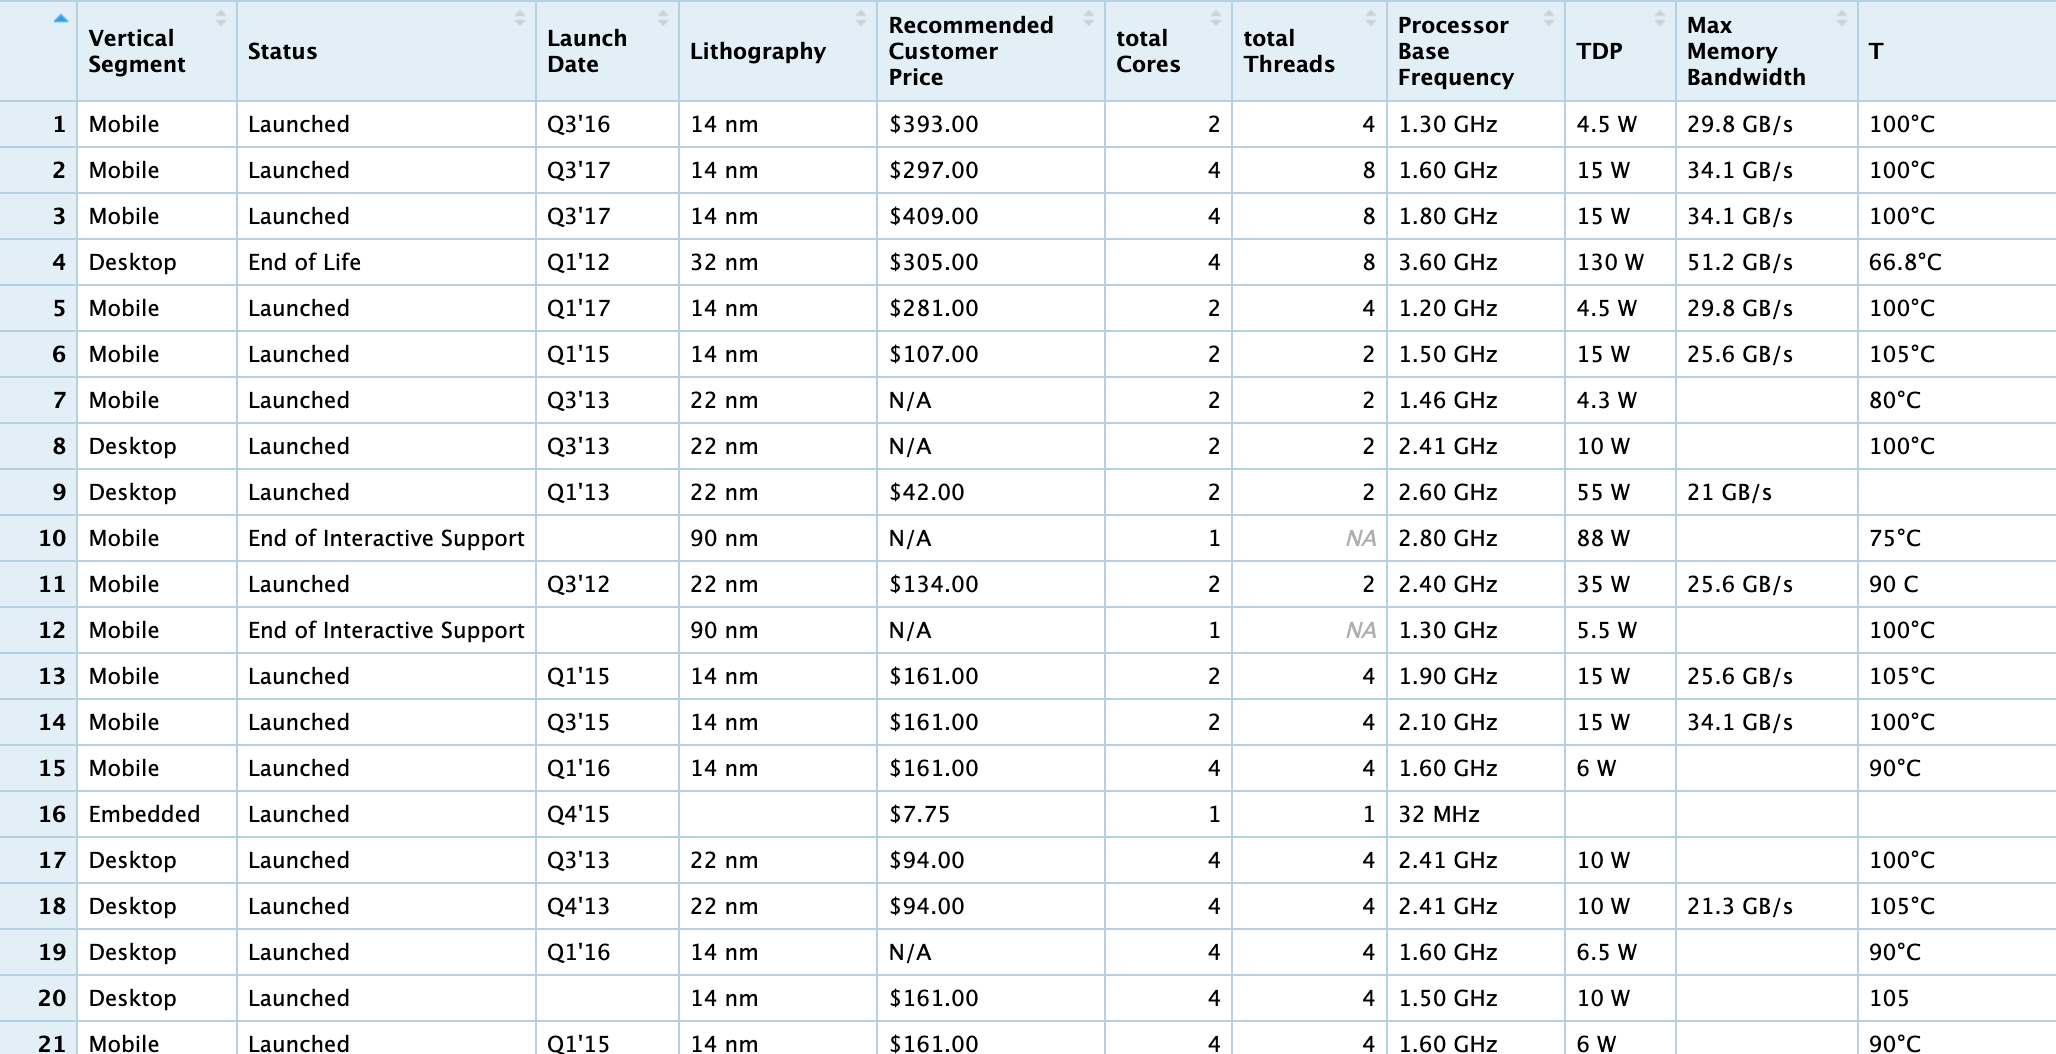
\includegraphics[max width=0.9\linewidth]{./graphics/short_data.png}
    \caption{Data before cleaning.}
\end{figure}

\subsubsection*{ldate}

\verb|market| and \verb|status| are left unchanged, since the values are straightforward. See \nameref{section:data_clarify} for further analysis.

The remaining attributes (columns) are processed as followed:

\inputcode[firstline=53,lastline=55]{R}{rcode/cleaning.r}

Our goal is to transform raw, non-standard string representation of year-quarter into \verb|zoo|'s standard representation. 
The function \mintinline{R}{as.yearqtr} takes a column and a format string as parameters. The format string is represented 
as: \mintinline{R}{"Q%q'%y"}, in which two flags \mintinline{R}{"%q"}, \mintinline{R}{"%y"} stands for quarter and year, respectively.
The format string hints the function to know the positions of quarter and year in our raw string.

\subsubsection*{litho}

\inputcode[firstline=62,lastline=64]{R}{rcode/cleaning.r}

Our goal is to cut out \verb|"nm"|, since every entry is recorded in nanometers anyway. \mintinline{R}{gsub} helps to replace a pattern 
of a string with another string. In this case, we replace any occurence of \verb|"nm"| with an empty string, and then cast the remaining 
value to numeric type. Notice that the pattern could be regular expression as well, this will be used intensively in the following cleaning
process.

\subsubsection*{rprice}

\inputcode[firstline=73,lastline=81]{R}{rcode/cleaning.r}

\textbf{HEY VIET TUNG WRITE THIS FOR ME THANK YOU!}
% YOU SHOULD EMBED THE BELOW LINE SOMEWHERE IN YOUR EXPLAINATION.
but the pattern is a regular expression (regex). Please refer to \nameref{section:appendix:regex}
for further information.

\subsubsection*{bfreq}

\inputcode[firstline=89,lastline=94]{R}{rcode/cleaning.r}

Our goal is to cut out \verb|"GHz"| and \verb|"MHz"| from the string, and convert all \verb|"MHz"| values into \verb|"GHz"|. Heuristically,
we observed that any value greater than 10 must be \verb|MHz|, so we can transform every value like that will be multiply by 0.001 to get 
the according \verb|MHz| value. \mintinline{R}{gsub} is used like as above. This time, that regex is used to match any substring that is 
\verb|GHz| OR \verb|MHz|. Then, we multiply with the 0.001 any number greater than 10, and store it back to the dataframe. Notice that the
\mintinline{R}{NA} values must be truncated first, as it is necessary to ensure dataframe subscripting to work.

\subsubsection*{tdp}

\inputcode[firstline=100,lastline=102]{R}{rcode/cleaning.r}

Our goal is to cut out \verb|"W"| from the string. The approach is similiar to the above.

\subsubsection*{memband}

\inputcode[firstline=108,lastline=110]{R}{rcode/cleaning.r}

Our goal is to cut out \verb|"GB/s"| from the string. The approach is similiar to the above.

\subsubsection*{temp}

\inputcode[firstline=124,lastline=133]{R}{rcode/cleaning.r}

Our goal is to only match the numeric values, then, take the maximum among those, since we are only interested in the maximum temperature.
This attribute's data are very varying in forms and the pattern we want is difficult if only a simple regular expression is used to match.
Our approach is can be described as follows:

\begin{itemize}
    \item First, we attempt to match every decimal numbers possible, including the irrelevant number. The rest are replaced with commas \verb|","|.
    
    The result of this process will create a string of numbers separated by commas. By doing this, the numbers are well isolated for our purpose.

    \item Second, we split these numbers and form a vector of them. This can be done through \mintinline{R}{strsplit} function. Notice that our numbers
    are still in string format.

    \item Third, we cast all these strings to numeric and push them into a vector of values using \mintinline{R}{unlist} and \mintinline{R}{lapply}
    
    \item Fourth, we find the maximum among all these values. Invalid numbers will automatically become \(-\infty\), and will be further treated as \mintinline{R}{NA}.

\end{itemize}

Notice that, we must loop through each row of the list to accomplish the above procedure.

Finally, the program produces \verb|cpu-clean.csv| as a cleaned data, ready for further exploitation in the later sections. This section uses a lot of regular expression
to match the desired strings, please refer to \nameref{section:appendix:regex} for more details.

\begin{figure}[H]
    \centering
    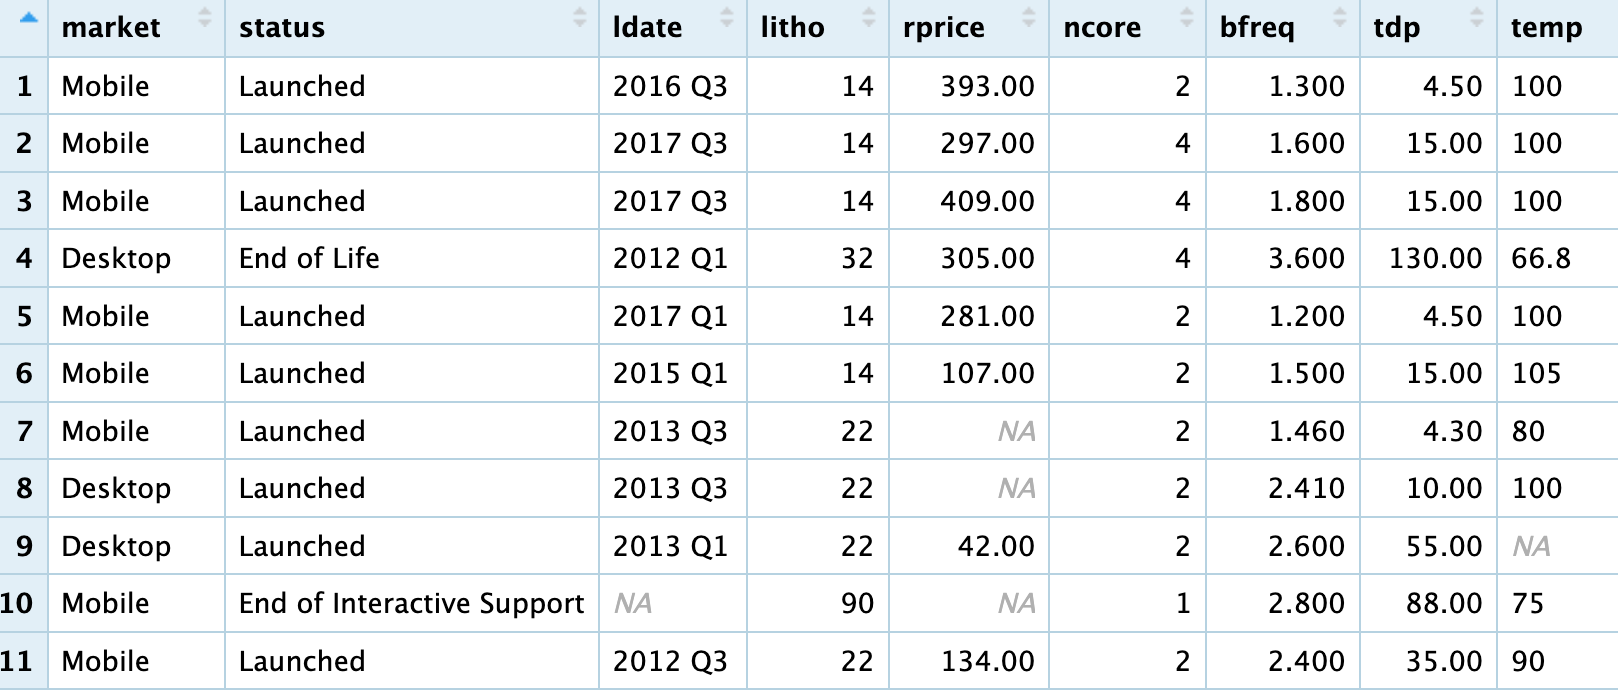
\includegraphics[max width=0.9\linewidth]{./graphics/cleaned_data.png}
    \caption{Data after cleaning.}
\end{figure}

% END OF DATA CLEANING